\documentclass[aps, 12pt]{revtex4}
\usepackage[english]{babel}
\usepackage[utf8]{inputenc}
\usepackage[T1]{fontenc}
% \usepackage{NotesTeX}
\usepackage{subfigure}
\usepackage{tikz}
\usetikzlibrary{arrows}
\usepackage{multirow}
\usepackage{listings}
\usepackage{extarrows}
\usepackage{parskip}
\usepackage{eurosym}
\usepackage{footmisc}
\usepackage{kantlipsum}
\usepackage{algorithm}
\usepackage{algpseudocode}


\def\thesection{\arabic{section}}

\renewcommand{\deg}{^{\circ}}
\newcommand\numberthis{\addtocounter{equation}{1}\tag{\theequation}}
\newcommand{\hksqrt}[2][]{\ \mathpalette\DHLhksqrt{[#1]{#2\,}}}
\def\DHLhksqrt#1#2{\setbox0=\hbox{$#1\sqrt#2$}\dimen0=\ht0
    \advance\dimen0-0.3\ht0
    \setbox2=\hbox{\vrule height\ht0 depth -\dimen0}
    {\box0\lower0.65pt\box2}}

\graphicspath{{figs/}}
\newcommand{\includegraphicsmaybe}[2][]{\IfFileExists{../plots/#2}{\includegraphics[#1]{#2}}{\includegraphics[width=0.7\linewidth]{giffel.jpg}}}



\begin{document}

\author{Håkon Olav Torvik}
\title{\Huge Problem Set 4 \\ \small Math228B Numerical solutions to differential equations}
\affiliation{UC Berkeley}
\date{\today}


\maketitle

\section*{Part 1}
Considering the bvp
\begin{align}
    u''''(x) = & f(x) \equiv 480x - 120, \hspace{3mm} x\in(0,1) \label{eq:diff}
    \\
    u(0) =     & u'(0) = u(1) = u'(1) = 0. \label{eq:boundary}
\end{align}
It is straight forward to find and verify that the analytical solution to \eqref{eq:diff}-\eqref{eq:boundary} is
\begin{equation*}
    u_{true}(x) = 4x^5 - 5x^4 - 2x^3 + 3x^2.
\end{equation*}

\subsection*{a}
A weighted average over the interval, for the approximate solution $u_h(x)\in V_h$, and for some function $v(x)$, is written as
\begin{equation*}
    \int_0^1u_h''''(x)v(x)dx = \int_0^1f(x)v(x)dx.
\end{equation*}
Simplifying by integrating by parts:
\begin{align*}
    \int_0^1u_h''''(x)v(x)dx & =u_h'''(x)v(x) \bigg\rvert_0^1 - \int_0^1u_h'''(x)v'(x)dx
    \\
                             & = \int_0^1u_h''(x)v''(x)dx + \bigg[ u_h'''(x)v(x)- u_h''(x)v'(x)\bigg]_0^1.
\end{align*}
By using the Galerkin method, we choose the function $v(x)$ to be from the same function space as $u_h(x)$, such that the boundary conditions \eqref{eq:boundary} are also imposed on $v(x)$. The last term above will then be 0, and we end up the problem being to find $u_h\in V_h$, such that
\begin{eqnarray} \label{eq:galerkin}
    \int_0^1u_h''(x)v''(x)dx = \int_0^1f(x)v(x)dx, \hspace{4mm} \forall v\in V_h
\end{eqnarray}

\subsection*{b}
Want to find a basis $\{\varphi_i\}$ that span
\begin{align*}
    V_h = \{v\in C^1([0,1]): v\vert_K\in\mathcal{P}_3(K)\forall K\in T_h, v(0)=v'(0)=v(1)=v'(1)=0\}.
\end{align*}
That is, we want a cubic on each of the 2 elements $K_i\in T_h = \{K_1, K_2\}$, giving 8 degrees of freedom. The 4 boundary conditions represents 4 constrains, while the continuity conditions $C^1$ are 2 further constraints, such that $\text{dim}(V_h)=2$.

To ensure orthogonality of the basis, I want basis functions that satisfy $\varphi_i^{(j)}(x)= \delta_{ij}, i,j=0, 1$, where $x=\frac{1}{2}$ is the only point in the domain where I'm free to choose any value of of the basis functions, and $f^{(k)}$ represents the kth derivative. I know that the cubic Hermite interpolating polynomials have the following properties:
\begin{align*}
    H_0(0)          & = 1 &  & \tilde{H}_0(0)=H_1(0)=\tilde{H}_1(0)=0 \\
    \tilde{H}'_0(0) & = 1 &  & H'_0(0)=H'_1(0)=\tilde{H}'_1(0)=0      \\
    H_1(1)          & = 1 &  & H_0(1)=\tilde{H}_0(1)=\tilde{H}_1(1)=0 \\
    \tilde{H}'_1(1) & = 1 &  & H'_0(1)=\tilde{H}'_0(1)=H'_1(1)=0      \\
\end{align*}

Then will $\{\varphi_0, \varphi_1\}$ form a basis for $V_h$, where
\begin{align*}
    \varphi_0 & =\begin{cases}
        H_1(2x)   & 0\leq x \leq \frac{1}{2}
        \\
        H_0(2x-1) & \frac{1}{2} < x \leq 1,
    \end{cases}
    \\
    \varphi_1 & =\begin{cases}
        \tilde{H}_1(2x)   & 0\leq x \leq \frac{1}{2}
        \\
        \tilde{H}_0(2x-1) & \frac{1}{2} < x \leq 1.
    \end{cases}
\end{align*}

\subsection*{c}
First I write the explicit expressions for the cubic Hermite polynomials and its derivatives for reference later.
\begin{align*}
    H_0(x)         & = 2x^3 - 3x^2 + 1 &  & H_0'(x) = 6x^2 - 6x         &  & H_0''(x) = 12x-6        \\
    H_1(x)         & = 3x^2-2x^3       &  & H_1'(x) = 6x-6x^2           &  & H_1''(x) = 6-12x        \\
    \tilde{H}_0(x) & = x^3-2x^2+x      &  & \tilde{H}_0'(x) = 3x^2-4x+1 &  & \tilde{H}_0''(x) = 6x-4 \\
    \tilde{H}_1(x) & = x^3-x^2         &  & \tilde{H}_1'(x) = 3x^2-2x   &  & \tilde{H}_1''(x) = 6x-2 \\
\end{align*}

From \eqref{eq:galerkin}, the solution $u$ to \eqref{eq:diff}-\eqref{eq:boundary} can be written
\begin{align*}
     & Au=b,                                                                                         \\
     & A_{ij}= \int_0^1\varphi_i''(x)\varphi_j''(x)dx, \hspace{4mm} b_i = \int_0^1f(x)\varphi_i(x)dx
\end{align*}

\newcommand{\io}{\int_0^{\frac{1}{2}}}
\renewcommand{\it}{\int_{\frac{1}{2}}^1}
\newcommand{\iu}{\frac{1}{2}\int_0^1}


To simplify integrals, I do the following change of variables.
\begin{align*}
    \io f(2x)dx   & = \iu f(x)dx
    \\
    \it f(2x-1)dx & = \iu f(x)dx
\end{align*}

Staring to integrate.
\begin{align*}
    A_{11}          & = \io H_1''(2x)^2dx + \it H_0''(2x-1)^2dx
    \\
                    & = \iu H_1''(x)^2dx + \iu H_0''(x)^2dx
    \\
    %                 & = \iu (6-12x)^2dx + \iu (12x-6)^2dx
    % \\
    %                 & = \iu (36 - 144x+144x^2)dx + \iu (144x^2-144x+36)dx
    % \\
    %                 & =\big[36x - 72x^2 + 48x^3]_0^1
    % \\
    %                 & = 36-72+48 = 12
                    & =12
    \\
    A_{22}          & = \io \tilde{H}_1''(2x)^2dx + \it \tilde{H}_0''(2x-1)^2dx
    \\
                    & = \iu \tilde{H}_1''(x)^2 + \iu \tilde{H}_0''(x)^2dx
    \\
    %                 & = \iu (6x-2)^2dx +\iu (6x-4)^2dx
    % \\
    %                 & = \iu (36x^2-24x+4)dx +\iu (36x^2-48x+16)dx
    % \\
    %                 & = \frac{1}{2}[12x^3-12x^2+4x]_0^1 +\frac{1}{2}[12x^3-24x^2+16x]_0^1
    % \\
    %                 & = \frac{1}{2}(12-12+4+12-24+16) = 4
                    & = 4
    \\
    A_{12} = A_{21} & = \io H_1''(2x)\tilde{H}_1''(2x)dx + \it H_0''(2x-1)\tilde{H}_0''(2x-1) dx
    \\
                    & = \iu H_1''(x)\tilde{H}_1''(x)dx +\iu H_0''(x)\tilde{H}_0''(x)dx
    \\
    %                 & = \iu (6-12x)(6x-2)dx + \iu (12x-6)(6x-4)dx
    % \\
    %                 & = \int_0^1 (18x-36x^2-6 + 12x)dx +\int_0^1(36x^2-24x-18x+12)dx
    % \\
    %                 & = (9-12-6+6) + (12-12-9+12) = 0
                    & = 0
    \\
    A               & =\begin{pmatrix}
        12 & 0 \\ 0 & 4
    \end{pmatrix}
    % \\
    % A^{-1}          & = 4^{-1}\frac{1}{3}\begin{pmatrix}
    %     1 & 0 \\ 0 & 3
    % \end{pmatrix} = \frac{1}{12}\begin{pmatrix}
    %     1 & 0 \\ 0 & 3
    % \end{pmatrix}
\end{align*}

\begin{align*}
    b_1 & = \io f(x)H_1(2x)dx + \it f(x)H_0(2x-1)dx
    \\
        & = \iu f\left(\frac{x}{2}\right)H_1(x)dx + \iu f\left(\frac{x+1}{2}\right)H_0(x)dx
    \\
        & = 60
    % \\
    %     & = \int_0^1 (120x-60)(3x^2-2x^3)dx + \int_0^1 (120x-180)(2x^3-3x^2+1)dx
    % \\
    %     & = \int_0^1(360x^3-240x^4-180x^2+120x^3)dx                                                         \\& \ \ \ \ + \int_0^1(240x^4-360x^3+120x-360x^3+540x^2-180)dx
    % \\
    %     & = (90-48-60+30) + (48-90+60-90+180-180)
    % \\
    %     & =12 -72 = -60
    \\
    b_2 & = \io f(x)\tilde{H}_1(2x)dx + \it f(x)\tilde{H}_0(2x-1)dx
    \\
        & = \iu f\left(\frac{x}{2}\right)\tilde{H}_1(x)dx + \iu f\left(\frac{x+1}{2}\right)\tilde{H}_0(x)dx
    % \\
    %     & = \int_0^1 (120x-60)(x^3-x^2)dx + \int_0^1(120x-180)(x^3-2x^2+x)dx
    % \\
    %     & =\int_0^1(120x^4-120x^3-60x^3+60x^2)dx                                                            \\ & \ \ \ \ + \int_0^1(120x^4-240x^3+120x^2-180x^3+360x^2-180x)
    % \\
    %     & = (24 - 60-15+20) + (24 - 60 +40 - 45 + 120 - 90)
    %     \\
    %     &= -27-11 = -38
    \\
        & = 8
    \\
    b   & = \begin{pmatrix}
        60 \\ 8
    \end{pmatrix}
\end{align*}
If I put this together to solve for $u$, I get that $u=\begin{pmatrix}
        5 \\ 2
    \end{pmatrix}$. Using these as coefficient for the basis functions I plot the numerical solution, along with the exact solution, in Figure \ref{fig:uplot}. My solution is obviously wrong, but due to time constraints I wasnt able to correct it. I think what I should have done was to not integrate over the whole domain, rather each element seperately, and get a $4\times 4$ matrix $A$, such that the solution $u$ has 4 coefficients, the first two being the coefficient for each basis function on $K_1$, and the second to on $K_2$. Because of the continuity constraint, these should be the same however, which is why I did not do this first.



\begin{figure}
    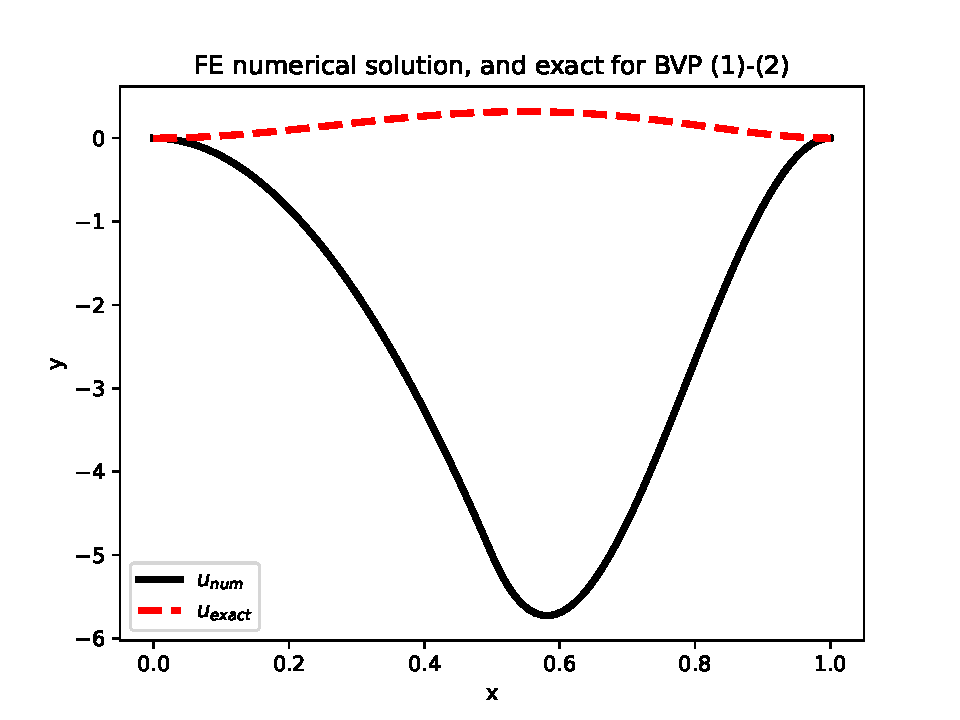
\includegraphics[width=\linewidth]{uplot.pdf}
    \caption{Numerical and exact solution. I obviously have found the wrong coefficients.}
    \label{fig:uplot}
\end{figure}

\section*{Part 2}

Using the stamping method as presented in the lecture notes, I write a function \texttt{fempoi()} for solving Poissons equation $-\nabla^2u= 1$ on any unstructured, triangulated mesh. Homogeneous dirichlet conditions are imposed on the edges, while homogeneous Neumann conditions naturally arise elsewhere.

Using this function, I recreate the 3 figures in the project description, in as part \textbf{a), b)} and \textbf{c)} in Figure \ref{fig:possions}. They all share a great resembelance with their counterpart.
For figure-balance I also include a solution on the square pac-man polygon from PS3, with dirichlet only on the 5 corners and Neumann along the edges, with methematically doesn't really make sense, but looks cool.

None of the meshes are refined. While testing, I found a bug in my meshgenerator from PS3, due to a misunderstainding of when to remove dengenerate triangles. This has been fixed in the code for this project.

\begin{figure}
    \minipage{0.5\textwidth}
    \textbf{a)}
    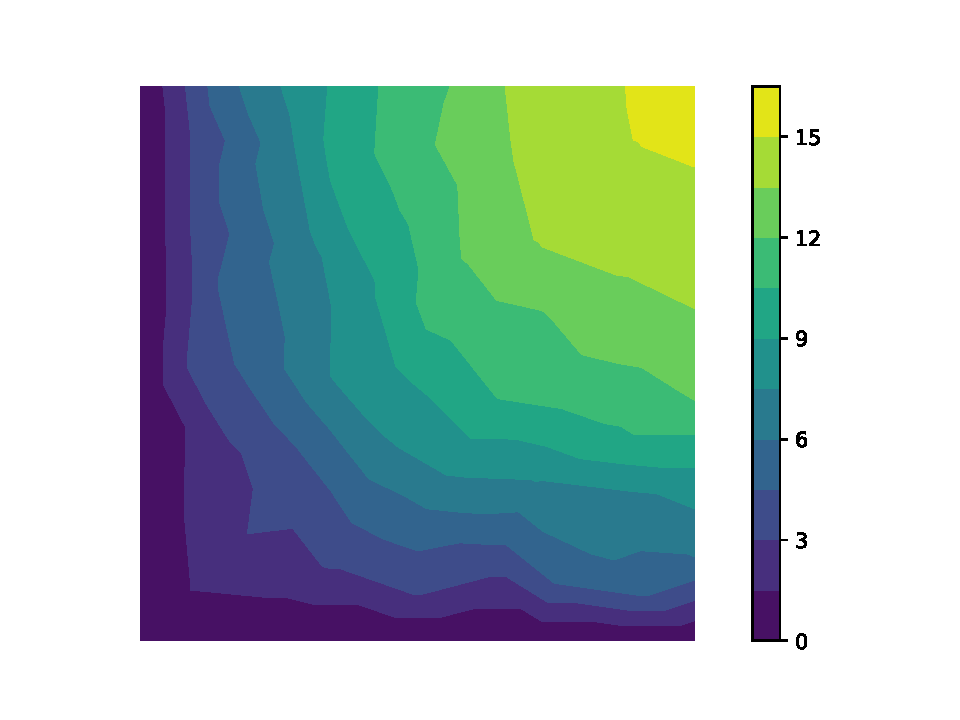
\includegraphics[width=\linewidth]{square.pdf}
    \endminipage\hfill
    \minipage{0.5\textwidth}
    \textbf{b)}
    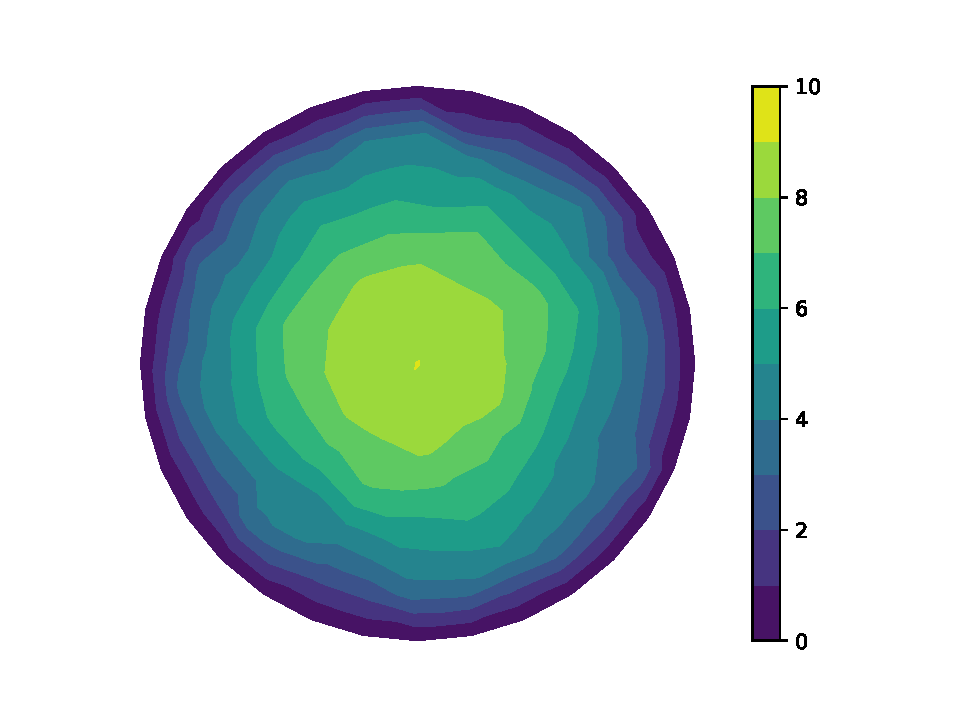
\includegraphics[width=\linewidth]{circle.pdf}
    \endminipage\hfill
    \minipage{0.5\textwidth}
    \textbf{c)}
    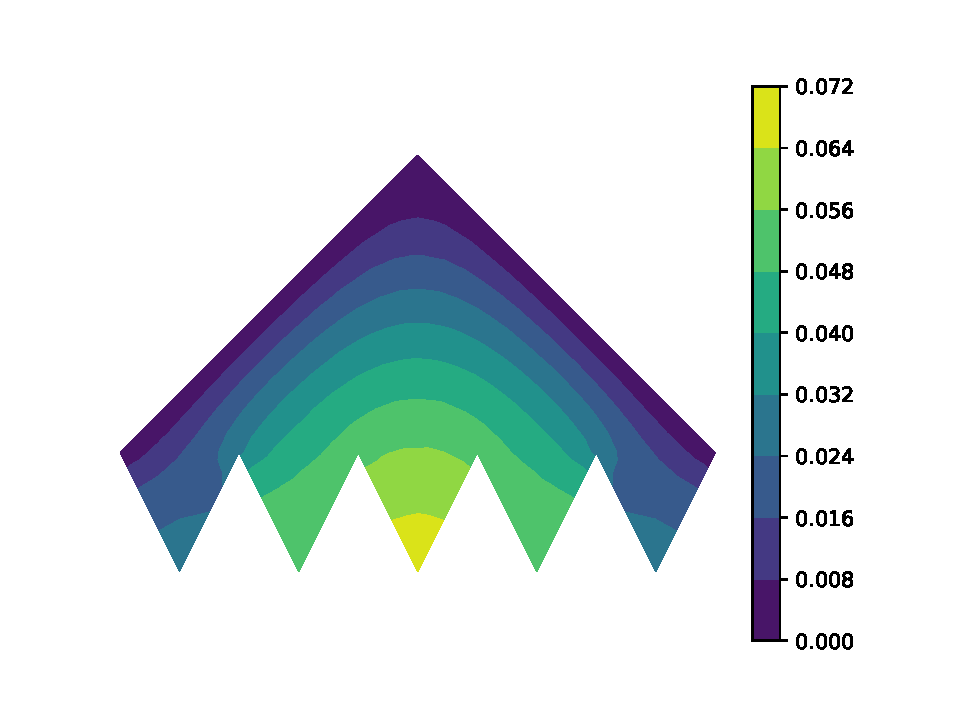
\includegraphics[width=\linewidth]{generic.pdf}
    \endminipage\hfill
    \minipage{.5\textwidth}
    \textbf{d)}
    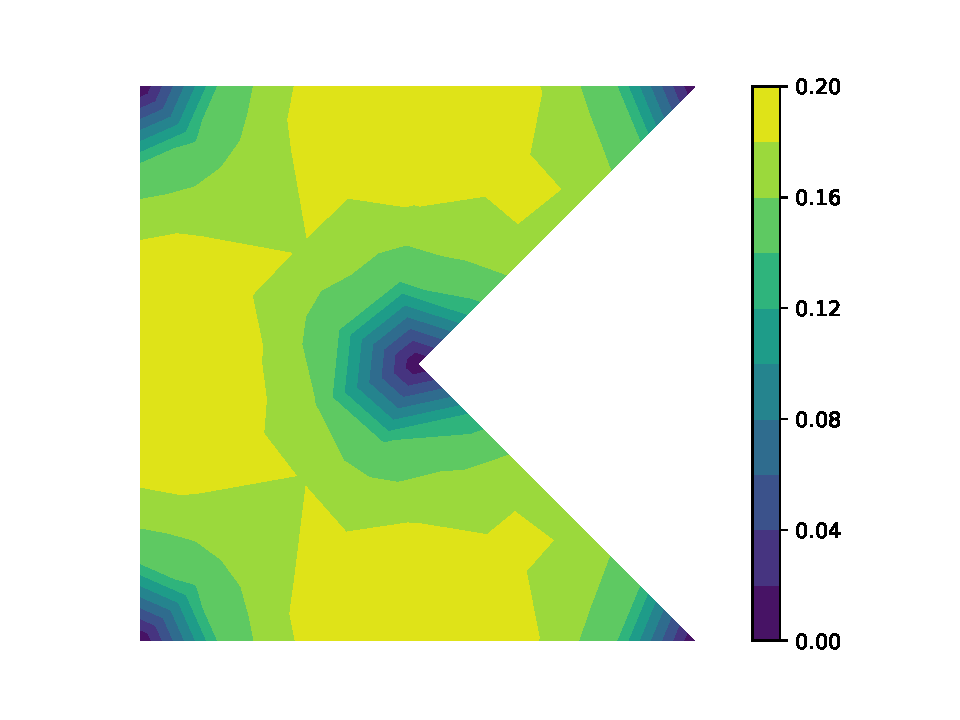
\includegraphics[width=\linewidth]{nepal.pdf}
    \endminipage\hfill
    \caption{Solution to poissions equation on each respective polygon, with a mix of dirichlet and neumann conditions. \textbf{a)}: Square, dirichlet on left and lower boundary. \textbf{b)}: circle, dirichlet on entire boundary. \textbf{c)}: jagged polygon, dirichlet on top. \textbf{d)}: Square pac-man, dirichlet on the 5 corners.}
    \label{fig:possions}
\end{figure}

\section*{Part 3}
To determine the convergence rate for the function \texttt{fempoi()}, I write a function \texttt{poiconv()} which calls \texttt{fempoi()} on a more and more refined mesh of the same polygon, and finds the max-norm of the difference between each refinement and the last.

To test this I use a square and a square pac-man (from PS3). The resulting convergence plot can be seen in Figure \ref{fig:conv}, where the true solution is taken as the 5th refinement of the mesh. From reading off the slope, we see that for the square the error goes as $\mathcal{O}(h^{2.12})$, while for the pac-man it goes as $\mathcal{O}(h^{1.14})$. The very same method is 2nd order accurate for one shape, while only 1st order accurate for another! This is because the constant in the error-bound is dependent on the angles of the triangles, and can be very large. This is the case for the square pac-man, and thus the method converges slower.

\begin{figure}
    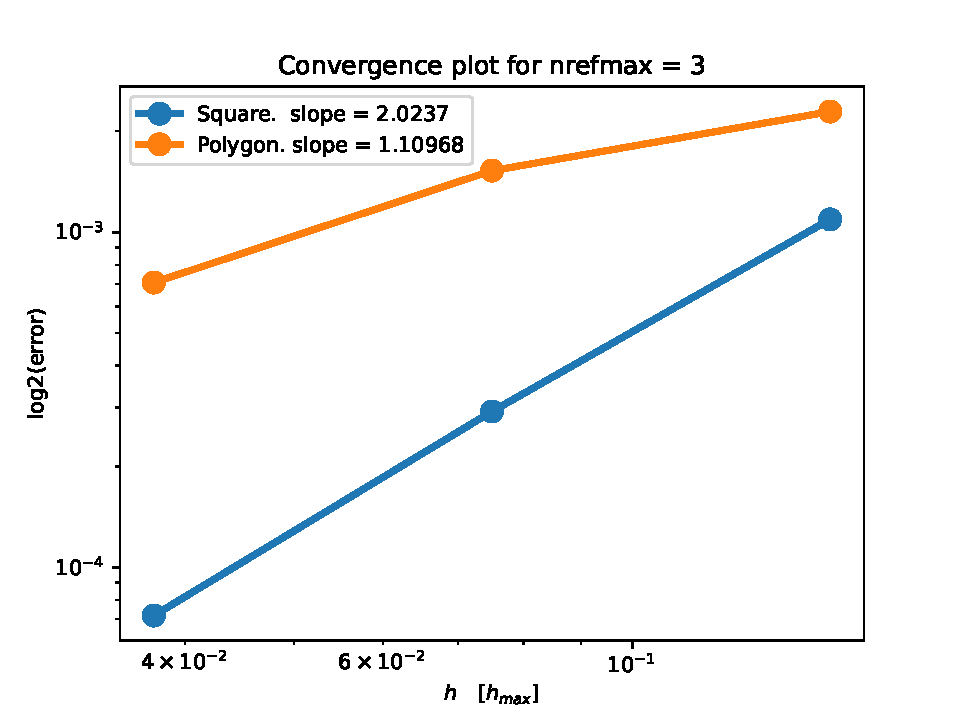
\includegraphics[width=\linewidth]{convplot.pdf}
    \caption{Convergence plot with rates for 2 different polygons, as function of refinement.}
    \label{fig:conv}
\end{figure}

\end{document}

